\documentclass[journal,twoside,web]{ieeecolor}
\usepackage{generic}
\usepackage{cite}
\usepackage{amsmath,amssymb,amsfonts}
\usepackage{algorithmic}
\usepackage{graphicx}
\usepackage{algorithm,algorithmic}
\usepackage{booktabs}
\usepackage{hyperref}
\hypersetup{hidelinks=true}
\usepackage{textcomp}
\def\BibTeX{{\rm B\kern-.05em{\sc i\kern-.025em b}\kern-.08em
    T\kern-.1667em\lower.7ex\hbox{E}\kern-.125emX}}
\markboth{\hskip25pc IEEE TRANSACTIONS AND JOURNALS}
{Zhang \MakeLowercase{\textit{et al.}}: HMC-GNN}
\begin{document}
\title{HMC-GNN: Gene-Overlap-Enhanced Multi-View Heterogeneous Graph Learning for Disease-Driven Herb Recommendation}
\author{Rongyun Zhang, Xiangping Wu, and Shengqiang Tong
\thanks{This work was supported by the National Natural Science Foundation of China under Grant 22478347 and the ``Pioneer'' and ``Leading Goose'' R\&D Project of Zhejiang Province under Grant 2025C04034.}
\thanks{Rongyun Zhang and Xiangping Wu are with the College of Information Engineering, China Jiliang University, Hangzhou 310018, China (e-mail: xiangpingwu@cjlu.edu.cn).}
\thanks{Xiangping Wu is also with the Zhejiang-New Zealand Joint Laboratory on Vision-Based Intelligent Metrology, Hangzhou 310018, China.}
\thanks{Shengqiang Tong is with the College of Pharmaceutical Science, Zhejiang University of Technology, Hangzhou 310014, China, and also with the Zhejiang Provincial Key Laboratory of TCM for Innovative R\&D and Digital Intelligent Manufacturing of TCM Great Health Products, Hangzhou 310014, China.}
\thanks{Corresponding author: Xiangping Wu.}}

\maketitle

\begin{abstract}
Disease-driven herb recommendation ranks candidate herbs for a disease query, but direct disease--herb supervision is sparse and external biomedical knowledge is often used only as static features or ordinary heterogeneous edges. This limits the ability of graph recommenders to convert gene-associated knowledge into recommendation-relevant structure and may mix local interactions, heterogeneous knowledge, and raw multimodal semantics in a single propagation space. We propose HMC-GNN, a gene-overlap-enhanced multi-view heterogeneous graph learning framework for disease-driven herb recommendation. HMC-GNN first computes shared-gene Jaccard similarity among diseases and among herbs to induce disease--disease and herb--herb semantic edges. It then separates representation learning into local, global, and semantic views: the local view captures disease--herb supervision and induced same-type neighborhoods, the global view models external heterogeneous knowledge, and the semantic view preserves projected multimodal node features without graph propagation. A gated fusion module integrates asymmetric herb and disease modalities, while graph self-supervision, graph--chemical alignment, and property--chemical alignment regularize the learned representations. On a constructed multimodal heterogeneous disease--herb graph under a disease-label-disjoint protocol, HMC-GNN achieves P@10 of 0.7044, R@10 of 0.2715, F1@10 of 0.2657, and NDCG@10 of 0.7829. Ablation and sensitivity analyses indicate that gene and chemical information, multi-view organization, and semantic residual fusion are important contributors. These results support a gene-aware multi-view graph learning framework for integrating traditional Chinese medicine semantics with biomedical knowledge.
\end{abstract}

\begin{IEEEkeywords}
Disease-driven herb recommendation, gene-overlap graph augmentation, heterogeneous graph neural network, multi-view learning, traditional Chinese medicine.
\end{IEEEkeywords}

\section{Introduction}
\label{sec:introduction}
\IEEEPARstart{T}{raditional} Chinese medicine (TCM) has developed a systematic view of disease prevention and treatment through long-term clinical practice \cite{ref1,ref2,ref3}. Unlike single-target therapeutic paradigms, TCM emphasizes holistic regulation and the coordinated use of multiple herbs with complementary properties, effects, and meridian tropisms \cite{ref4,ref5,ref6,ref7}. With the increasing availability of structured TCM knowledge bases and biomedical resources, computational herb recommendation has become an important task for supporting intelligent TCM analysis and integrative medicine research \cite{ref8,ref9,ref10}.

Most existing computational studies on TCM recommendation focus on symptom-driven or prescription-driven scenarios, where a relatively rich set of symptoms, syndromes, or historical prescriptions is available as input \cite{ref11,ref12}. In these settings, models can exploit dense symptom--herb co-occurrence patterns or formula-level composition signals to infer candidate herbs. However, in many integrative medicine scenarios, the available query may be a disease diagnosis rather than a detailed symptom profile \cite{ref13,ref14,ref15}. This gives rise to disease-driven herb recommendation, where the goal is to rank candidate herbs for a given disease query. Compared with symptom-driven recommendation, this setting is more challenging because the disease input is sparse and directly observed disease--herb supervision is insufficient for robust generalization \cite{ref16,ref17}. The key problem is therefore not merely the difference between disease and symptom inputs, but how to transform sparse disease--herb labels and external biomedical knowledge into useful recommendation structure.

Graph-based methods provide a natural framework for modeling heterogeneous TCM knowledge. By representing diseases, herbs, properties, effects, chemicals, and other entities as nodes, heterogeneous graph neural networks can aggregate information across multiple relation types and capture high-order dependencies \cite{ref35,ref36,ref11,ref38,ref39,ref40,ref41}. Nevertheless, existing graph-based recommendation methods still face several limitations in disease-driven herb recommendation. First, many methods mainly rely on direct co-occurrence or observed disease--herb relations. When supervision is sparse, such topology may fail to provide sufficient signals for rare diseases or less frequent herbs, and dense collaborative connections can further introduce popularity bias and over-smoothing during graph propagation \cite{ref42,ref43,ref44}. Second, external biomedical knowledge, such as disease--gene and herb--gene associations, is often used only as node attributes or ordinary heterogeneous edges. This strategy enriches node information, but it does not explicitly convert gene-level associations into local semantic neighborhoods that are directly useful for recommendation. Third, local recommendation interactions, global heterogeneous knowledge, and raw multimodal node semantics are often propagated in a unified graph. Such unified propagation may mix semantically different signals and weaken discriminative representation learning.

To address these challenges, we propose HMC-GNN, a Heterogeneous Multi-view Contrastive Graph Neural Network for disease-driven herb recommendation. The central idea is to transform external gene associations into recommendation-relevant local semantic topology while separately learning complementary local, global, and semantic views. Specifically, disease--gene and herb--gene associations are first converted into gene sets for diseases and herbs. We then compute shared-gene Jaccard similarities among same-type nodes and construct disease--disease and herb--herb gene-overlap semantic edges. These induced edges provide local semantic neighborhoods beyond directly observed disease--herb labels, allowing recommendation signals to propagate among semantically related diseases and herbs. Importantly, these gene-overlap edges are used as semantic associations for representation learning rather than as evidence of causal therapeutic mechanisms.

Beyond graph augmentation, HMC-GNN adopts a complementary multi-view learning architecture. The local view captures disease--herb supervision and induced local similarity relations, including co-label similarity and gene-overlap semantic edges. The global view models external heterogeneous knowledge, such as herb--chemical, herb--effect, herb--property, herb--meridian, disease--gene, and herb--gene relations. The semantic view preserves projected multimodal node features without graph propagation, thereby retaining node-level information that may be diluted during multi-hop message passing. Separate encoders are used for the local and global graph views, while the semantic view is encoded by a feature projection module. A semantic residual path further injects node-level multimodal semantics into graph-based representations to reduce semantic dilution during graph propagation.

HMC-GNN also introduces gated multimodal fusion to handle the asymmetric modality structures of diseases and herbs. Herb nodes integrate structural signals, TCM attribute semantics, chemical information, and gene features, whereas disease nodes integrate structural signals, textual features, and gene features. A single additive fusion strategy may mix incompatible modalities and weaken type-specific semantics. Therefore, HMC-GNN applies modality-level and view-level gating to adaptively integrate heterogeneous signals for diseases and herbs. The model is optimized with a joint objective that combines Bayesian Personalized Ranking (BPR) for the primary recommendation task with graph self-supervision, graph--chemical alignment, and property--chemical semantic alignment \cite{ref51,ref52}. These auxiliary objectives regularize the learned representations across structural, chemical, and TCM semantic spaces.

The main contributions of this work are summarized as follows:

\begin{itemize}
\item We propose a gene-overlap-guided local semantic graph augmentation strategy for disease-driven herb recommendation. By computing shared-gene Jaccard similarities among diseases and among herbs, HMC-GNN constructs disease--disease and herb--herb semantic edges, transforming gene associations from static side information into recommendation-relevant local topology.
\item We design a complementary local--global--semantic view learning framework. The local view captures recommendation-specific interactions and induced semantic neighborhoods, the global view captures external heterogeneous knowledge, and the semantic view preserves raw multimodal node information. A semantic residual path further alleviates semantic dilution during graph propagation.
\item We introduce gated multimodal fusion and contrastive alignment for asymmetric disease and herb representations. Herb nodes integrate structural, TCM semantic, chemical, and gene signals, while disease nodes integrate structural, textual, and gene signals. The model is jointly optimized with ranking, graph self-supervision, graph--chemical alignment, and property--chemical semantic alignment objectives.
\item We evaluate HMC-GNN under a disease-label-disjoint protocol, where validation and test disease--herb labels are excluded from the training graph. Experimental results, ablation studies, and sensitivity analyses examine the contribution of gene-overlap local semantic augmentation, multi-view encoding, semantic residual learning, and gated fusion for top-$K$ disease-driven herb recommendation.
\end{itemize}

\section{Related Work}
\label{sec:related_work}

\subsection{TCM Herb and Prescription Recommendation}

Computational TCM herb recommendation has been studied through statistical modeling, neural generation, and graph-based recommendation. Early statistical and topic-modeling methods treat prescriptions as documents and symptoms or herbs as words, aiming to discover latent therapeutic topics and co-occurrence patterns from historical records \cite{ref21,ref22,ref23,ref24,ref25}. Knowledge-enhanced topic models further incorporate structured relations into probabilistic prescription modeling \cite{ref26}. These methods provide interpretable statistical associations, but they are less suited to modeling higher-order dependencies among heterogeneous entities such as diseases, herbs, effects, chemicals, and genes.

Neural prescription models were later introduced to capture richer symptom--herb mappings. Sequence-based methods formulate prescription generation as a sequence-to-sequence task and use recurrent or Transformer-based architectures to map symptom descriptions to herb sequences \cite{ref27,ref29,ref30,ref31,ref32,ref33,ref34}. Feature-fusion approaches such as PresRecRF further integrate large-scale TCM semantics and molecular knowledge to improve prescription recommendation \cite{ref28}. These models expand the representational capacity of prescription recommendation, but many of them are designed for symptom-set or formula-generation settings. Because herbal prescriptions are unordered combinations rather than strict sequences, sequence modeling may also underrepresent set-level compatibility and multi-relational dependencies.

Graph-based TCM recommendation methods model symptoms, herbs, syndromes, effects, formulas, or related entities as structured graphs. Representative studies such as SMGCN and KDHR use graph convolution or multi-layer information fusion to learn symptom--herb or disease--herb representations \cite{ref36,ref11,ref38}. Subsequent models incorporate multi-graph aggregation, heterogeneous graph construction, residual attention, or semantic knowledge fusion to strengthen recommendation representations \cite{ref39,ref40,ref41,ref55}. These studies show that graph learning is a strong foundation for TCM recommendation. However, most existing methods are still centered on symptom-driven prescription recommendation or formula-level recommendation. HMC-GNN instead focuses on disease-driven herb ranking, where the query is a disease node and the directly observed disease--herb supervision is sparse. The goal is therefore not to reproduce the full syndrome differentiation or formula generation process, but to convert external biomedical and multimodal knowledge into recommendation-relevant graph structure.

\subsection{Knowledge-Aware Graph Recommendation}

Knowledge-aware recommendation incorporates external structured knowledge to enrich query and candidate representations. In general recommendation scenarios, knowledge graphs are commonly used to introduce semantic relations, alleviate data sparsity, and improve interpretability. These methods can be broadly divided into knowledge graph embedding-based methods and graph neural network-based methods. Knowledge graph embedding methods learn low-dimensional entity and relation representations through translational, bilinear, or neural scoring functions, which can then be combined with recommendation objectives. Although these methods capture global relational patterns, they are less flexible for modeling task-specific local topology and multimodal node attributes.

Graph neural network-based recommenders directly perform message passing over user--item graphs or heterogeneous knowledge graphs. Graph convolutional networks, graph attention networks, and relation-aware variants aggregate neighborhood information to capture high-order collaborative and semantic signals \cite{ref35,ref43,ref44}. In heterogeneous graph recommendation, relation-aware propagation is particularly important because different edge types encode different meanings. RGCN-style propagation is therefore suitable for modeling multi-relational graphs involving diseases, herbs, genes, chemicals, and TCM semantic entities.

Despite their effectiveness, existing knowledge-aware graph recommenders often treat external knowledge as ordinary side-information edges. In disease-driven herb recommendation, disease--gene and herb--gene associations contain useful biomedical semantics, but simply adding them as heterogeneous edges does not fully exploit their relevance to recommendation. Shared gene associations can induce local semantic neighborhoods among diseases and among herbs, offering a way to connect sparse disease--herb labels through same-type similarity. HMC-GNN follows this insight by transforming gene associations into disease--disease and herb--herb semantic topology, rather than using gene information only as node attributes or generic graph edges.

\subsection{Multi-View and Multimodal Graph Learning}

Multi-view and multimodal graph learning aims to integrate complementary information from different structures, modalities, or semantic spaces. In biomedical and TCM-related applications, available information is naturally heterogeneous, including structured relations, textual descriptions, TCM attributes, chemical components, molecular fingerprints, and gene associations \cite{ref45,ref46,ref47,ref48,ref49,ref50}. Existing multimodal TCM recommendation methods commonly fuse such information through concatenation, attention, or gating. These strategies demonstrate the value of combining macroscopic TCM semantics with microscopic biomedical or molecular information, but they often assume a relatively uniform feature structure across entity types or focus mainly on herb-side features.

Disease-driven herb recommendation has asymmetric modality availability. Herb nodes may be associated with TCM attributes, chemical features, and gene features, whereas disease nodes mainly have textual descriptions and gene associations. A single shared fusion mechanism may therefore mix incompatible modalities and weaken type-specific semantics. Moreover, propagating local recommendation interactions, global heterogeneous knowledge, and raw multimodal features in one unified graph may dilute node-level semantics during multi-hop aggregation. HMC-GNN addresses this issue through complementary local, global, and semantic views. The local view captures disease--herb supervision and induced same-type semantic neighborhoods, the global view captures external heterogeneous knowledge, and the semantic view preserves projected multimodal node features without graph propagation. This design distinguishes HMC-GNN from prior graph and multimodal recommendation methods by combining gene-overlap local semantic augmentation with view-level and modality-level gated fusion.

\section{Methodology}
\label{sec:methodology}

\subsection{Problem Formulation}
\label{subsec:problem_formulation}

We formulate disease-driven herb recommendation as a top-$K$ ranking problem on a multimodal heterogeneous disease--herb graph. Given a disease query, the task is to rank candidate herbs according to their potential relevance to the disease. Unlike symptom-driven prescription recommendation, the input in this setting is a disease node rather than a rich symptom or syndrome set. The model therefore needs to learn from sparse disease--herb supervision while using external heterogeneous knowledge and multimodal node semantics as side information.

Let $\mathcal{D}=\{d_1,d_2,\ldots,d_{|\mathcal{D}|}\}$ denote the disease nodes and $\mathcal{H}=\{h_1,h_2,\ldots,h_{|\mathcal{H}|}\}$ denote the candidate herb nodes. The heterogeneous graph also contains gene nodes $\mathcal{G}$, chemical component nodes $\mathcal{C}$, and TCM semantic nodes $\mathcal{A}$, where $\mathcal{A}$ includes effect, property/flavor, and meridian-related entities. The overall node set is
\begin{equation}
\mathcal{V}=\mathcal{D}\cup\mathcal{H}\cup\mathcal{G}\cup\mathcal{C}\cup\mathcal{A}.
\label{eq:node_set}
\end{equation}
The graph is denoted by $\mathcal{G}_{\mathrm{het}}=(\mathcal{V},\mathcal{E},\mathcal{R})$, where $\mathcal{E}$ is the set of typed edges and $\mathcal{R}$ is the set of relation types. The primary supervision is the observed disease--herb association set $\mathcal{Y}\subseteq \mathcal{D}\times\mathcal{H}$, which is used as implicit positive feedback. In addition, the graph contains external relations including disease--gene, herb--gene, herb--chemical, herb--effect, herb--property/flavor, and herb--meridian relations.

For each disease $d\in\mathcal{D}$, let $\mathcal{H}_d^{+}$ be the set of observed positive herbs. HMC-GNN learns a scoring function $s(d,h)$ for each disease--herb pair $(d,h)$, where $h\in\mathcal{H}$. After representation learning, the final disease and herb embeddings are denoted by $\mathbf{z}_d$ and $\mathbf{z}_h$, and the matching score is computed as
\begin{equation}
s(d,h)=\mathbf{z}_d^{\top}\mathbf{z}_h .
\label{eq:score}
\end{equation}
For each disease query, all candidate herbs are ranked by $s(d,h)$, and the top-$K$ herbs are returned.

Because only positive disease--herb associations are observed, training follows an implicit-feedback ranking setting. For each observed pair $(d,h^{+})$, a negative herb $h^{-}$ is sampled from $\mathcal{H}\setminus\mathcal{H}_d^{+}$. The primary ranking objective is the Bayesian Personalized Ranking (BPR) loss \cite{ref51}:
\begin{equation}
\mathcal{L}_{\mathrm{BPR}}
=-\sum_{(d,h^{+},h^{-})\in\mathcal{O}}
\log \sigma\left(s(d,h^{+})-s(d,h^{-})\right),
\label{eq:bpr}
\end{equation}
where $\sigma(\cdot)$ is the sigmoid function and $\mathcal{O}$ denotes the sampled training triples.

To reduce label leakage, we use a disease-label-disjoint evaluation protocol. Diseases are split into training, validation, and test groups at the disease level. During training-graph construction, only disease--herb labels associated with training diseases are inserted as supervision edges, whereas validation and test disease--herb labels are held out for evaluation. External side information, including disease text, disease--gene associations, herb--gene associations, herb--chemical relations, and TCM semantic relations, remains available. This protocol evaluates whether the model can recommend herbs for diseases whose recommendation labels are unseen during training, while still allowing access to external semantic knowledge associated with those diseases.

\subsection{Overview of HMC-GNN}
\label{subsec:method_overview}

HMC-GNN is designed to learn disease and herb representations from three complementary sources: local recommendation topology, global heterogeneous knowledge, and raw multimodal node semantics. Instead of propagating all relations and features in a single graph, HMC-GNN separates them into a local view, a global view, and a semantic view. The local view captures disease--herb supervision and induced same-type semantic relations. The global view models external heterogeneous knowledge. The semantic view preserves projected multimodal node features without graph propagation.

The framework contains four main components. First, a gene-overlap local semantic graph augmentation module converts disease--gene and herb--gene associations into disease--disease and herb--herb semantic edges. Second, view-specific relational graph convolutional network (RGCN) encoders aggregate information separately from the local and global views. Third, a semantic branch encodes multimodal node features and injects them into graph-based representations through semantic residual connections. Fourth, type-aware modality and view fusion modules generate final disease and herb embeddings for top-$K$ recommendation.

\subsection{Gene-Overlap Local Semantic Graph Augmentation}
\label{subsec:gene_overlap}

Disease--gene and herb--gene associations provide biomedical semantics, but treating them only as ordinary heterogeneous edges does not explicitly create recommendation-oriented neighborhoods among diseases or among herbs. HMC-GNN therefore transforms gene associations into same-type local semantic topology. For each disease or herb node, we first collect its associated gene set. Given two same-type nodes $i$ and $j$, with gene sets $\mathcal{G}_i$ and $\mathcal{G}_j$, their gene-overlap similarity is computed by the Jaccard coefficient:
\begin{equation}
J(i,j)=\frac{|\mathcal{G}_i\cap\mathcal{G}_j|}
{|\mathcal{G}_i\cup\mathcal{G}_j|}.
\label{eq:jaccard}
\end{equation}
A larger $J(i,j)$ indicates stronger shared gene-level annotation between two diseases or two herbs.

Based on this similarity, HMC-GNN constructs disease--disease and herb--herb gene-overlap semantic edges. Candidate same-type neighbors are filtered by shared-gene constraints and Jaccard similarity, followed by percentile-based sparsification and bounded neighborhood selection to avoid overly dense local graphs. The retained high-overlap disease pairs and herb pairs are added to the local view as gene-overlap semantic relations. These edges are used as semantic associations for representation learning, not as evidence of causal therapeutic mechanisms.

\subsection{Local, Global, and Semantic Views}
\label{subsec:views}

The local view is designed to carry recommendation-specific signals. It contains observed disease--herb training labels and their reverse edges, together with same-type similarity edges induced from co-label overlap and gene-overlap similarity. Herb--herb disease-overlap edges are induced from shared associated diseases, whereas disease--disease herb-overlap edges are induced from shared associated herbs. Together with the gene-overlap relations in Section~\ref{subsec:gene_overlap}, these edges form a local semantic topology for recommendation-oriented message propagation.

The global view contains external heterogeneous knowledge after excluding local recommendation and similarity relations. It includes herb--chemical, herb--effect, herb--property/flavor, herb--meridian, disease--gene, and herb--gene relations. This view provides broad TCM semantic, chemical, and gene-associated information that complements the local recommendation topology.

The semantic view consists of projected multimodal node features without graph propagation. It is introduced to preserve node-level semantic information that may be diluted during multi-hop message passing. For herb nodes, the semantic view integrates TCM attribute information, component-based features, chemical embeddings or fingerprints, and gene features. For disease nodes, it integrates disease text features and gene features. Auxiliary nodes are represented by learnable embeddings or available projected features. This view serves as a direct semantic reference for graph-based representations.

\subsection{View-Specific Encoding and Semantic Residual}
\label{subsec:encoding}

The local and global views are encoded by two independent RGCN stacks. Given initial node representations $\mathbf{X}$ and local-view edges $\mathcal{E}_{\mathrm{local}}$, the local encoder computes
\begin{equation}
\mathbf{Z}_{\mathrm{local}}
=\mathrm{RGCN}_{\mathrm{local}}(\mathbf{X},\mathcal{E}_{\mathrm{local}}).
\label{eq:local_rgcn}
\end{equation}
Similarly, for global-view edges $\mathcal{E}_{\mathrm{global}}$, the global encoder computes
\begin{equation}
\mathbf{Z}_{\mathrm{global}}
=\mathrm{RGCN}_{\mathrm{global}}(\mathbf{X},\mathcal{E}_{\mathrm{global}}).
\label{eq:global_rgcn}
\end{equation}
Separating the two encoders prevents recommendation-specific local topology and broad external knowledge from being forced into one message-passing channel.

The semantic view is encoded by a projection network:
\begin{equation}
\mathbf{Z}_{\mathrm{sem}}=\mathrm{MLP}(\mathbf{X}_{\mathrm{sem}}),
\label{eq:semantic_projection}
\end{equation}
where $\mathbf{X}_{\mathrm{sem}}$ denotes the projected multimodal semantic features. To reduce semantic dilution in graph propagation, HMC-GNN injects the semantic representation into both graph streams:
\begin{equation}
\widetilde{\mathbf{Z}}_{\mathrm{local}}
=\mathbf{Z}_{\mathrm{local}}+\beta\mathbf{Z}_{\mathrm{sem}},
\quad
\widetilde{\mathbf{Z}}_{\mathrm{global}}
=\mathbf{Z}_{\mathrm{global}}+\beta\mathbf{Z}_{\mathrm{sem}},
\label{eq:semantic_residual}
\end{equation}
where $\beta$ controls the strength of the semantic residual path.

\subsection{Type-Aware Fusion and Recommendation Scoring}
\label{subsec:fusion_scoring}

Disease and herb nodes have asymmetric modality structures. Herb nodes contain TCM attributes, chemical information, and gene features, whereas disease nodes mainly contain textual and gene-associated information. HMC-GNN therefore uses type-aware modality fusion before graph encoding. Herb-related modalities are projected into a shared latent space and fused by a herb-specific gate, while disease-related modalities are projected and fused by a disease-specific gate. This produces initial representations with a unified embedding dimension while preserving node-type-specific semantic composition.

After view-specific encoding, HMC-GNN applies type-aware view fusion to combine the local, global, and semantic representations. For a herb node, a herb-specific gate adaptively combines $\widetilde{\mathbf{Z}}_{\mathrm{local}}$, $\widetilde{\mathbf{Z}}_{\mathrm{global}}$, and $\mathbf{Z}_{\mathrm{sem}}$. For a disease node, a disease-specific gate combines the same three views with parameters specific to disease nodes. The fused representations are used as the final embeddings $\mathbf{z}_h$ and $\mathbf{z}_d$ for scoring in Eq.~\eqref{eq:score}.

\subsection{Multi-Objective Optimization}
\label{subsec:optimization}

HMC-GNN is optimized by combining the primary ranking objective with auxiliary self-supervised and semantic alignment losses:
\begin{equation}
\mathcal{L}
=\mathcal{L}_{\mathrm{BPR}}
+\lambda_{\mathrm{g}}\mathcal{L}_{\mathrm{GraphSSL}}
+\lambda_{\mathrm{c}}\mathcal{L}_{\mathrm{CrossModal}}
+\lambda_{\mathrm{p}}\mathcal{L}_{\mathrm{PropertyChemical}}.
\label{eq:total_loss}
\end{equation}
The BPR loss drives disease--herb ranking. The graph self-supervised loss encourages consistency of node representations under graph perturbations \cite{ref52}. The cross-modal alignment loss aligns graph-based herb representations with chemical semantic representations, and the property--chemical alignment loss encourages consistency between macroscopic TCM attribute semantics and microscopic chemical semantics. These auxiliary objectives regularize the representation space while the ranking loss remains the primary supervision for herb recommendation.

\section{Experiments}
\label{sec:experiments}

\subsection{Experimental Setup}
\label{subsec:experimental_setup}

\subsubsection{Dataset}
\label{subsubsec:dataset}

We evaluated HMC-GNN on a constructed multimodal heterogeneous disease--herb graph for disease-driven herb recommendation. The graph contains diseases, herbs, genes, chemical components, and TCM semantic entities, including effects, properties/flavors, and meridian tropisms. Disease--herb associations provide the primary recommendation supervision, whereas disease--gene, herb--gene, herb--chemical, herb--effect, herb--property/flavor, and herb--meridian relations provide external heterogeneous knowledge.

The final graph contains 17,683 nodes, 18 relation types, and 719,081 typed edges. The candidate set contains 395 herbs. To reduce label leakage, we used a disease-label-disjoint evaluation protocol. Diseases were split at the disease level into 2,162 training diseases, 270 validation diseases, and 271 test diseases. Only disease--herb labels from training diseases were inserted into the training graph. Disease--herb labels from validation and test diseases were excluded from graph construction and used only for evaluation. The numbers of disease--herb label edges in the training, validation, and test sets were 203,815, 22,547, and 22,468, respectively.

This protocol is not a fully inductive unseen-node setting. External side information, including disease text, disease--gene associations, herb--gene associations, herb--chemical relations, and TCM semantic relations, remains available for validation and test diseases. The protocol therefore evaluates generalization to diseases whose recommendation labels are unseen during training, while still allowing the model to use their available biomedical and TCM semantic side information.

\subsubsection{Baselines}
\label{subsubsec:baselines}

We compared HMC-GNN with representative recommendation baselines under the same candidate herb set and disease-label-disjoint evaluation protocol. The comparison included basic collaborative filtering models, namely BPR-MF \cite{ref51} and LightGCN \cite{ref56}, and adapted TCM recommendation baselines, including PresRecRF-style \cite{ref28}, KDHR-style \cite{ref38}, and BSGAM-style models. For baselines originally designed for symptom-driven or prescription-driven recommendation, we adapted the input to the disease-driven setting and prevented validation and test disease--herb labels from entering the training graph. These adapted baselines should be interpreted as fair disease-driven implementations of their core modeling ideas, rather than exact reproductions of their original experimental settings.

\subsubsection{Evaluation Metrics}
\label{subsubsec:metrics}

We evaluated top-$K$ herb recommendation using Precision@K, Recall@K, F1@K, and NDCG@K, with $K\in\{5,10,20,50\}$. For a disease $d$, let $\widehat{\mathcal{H}}_K(d)$ denote the top-$K$ recommended herbs and let $\mathcal{H}^{*}(d)$ denote the ground-truth herb set. The metrics are defined as
\begin{align}
\mathrm{P}@K &= \frac{|\widehat{\mathcal{H}}_K(d)\cap\mathcal{H}^{*}(d)|}{K}, \label{eq:precision}\\
\mathrm{R}@K &= \frac{|\widehat{\mathcal{H}}_K(d)\cap\mathcal{H}^{*}(d)|}{|\mathcal{H}^{*}(d)|}, \label{eq:recall}\\
\mathrm{F1}@K &= \frac{2\cdot \mathrm{P}@K\cdot \mathrm{R}@K}{\mathrm{P}@K+\mathrm{R}@K}, \label{eq:f1}\\
\mathrm{NDCG}@K &= \frac{1}{\mathrm{IDCG}@K}\sum_{r=1}^{K}\frac{\mathbf{1}(\hat{h}_r\in\mathcal{H}^{*}(d))}{\log_2(r+1)}. \label{eq:ndcg}
\end{align}
Because disease--herb labels are binary and do not contain graded clinical importance, NDCG@K was computed with binary relevance. Final values were averaged over all test diseases.

\subsubsection{Implementation Details}
\label{subsubsec:implementation}

HMC-GNN was implemented in PyTorch and optimized with Adam. The embedding dimension and hidden dimension were both set to 256. The batch size was 1024, the learning rate was $1\times10^{-3}$, the weight decay was $1\times10^{-5}$, and dropout was set to 0.2. The maximum number of epochs was 800, with early stopping patience of 20 validation evaluations. The graph self-supervised temperature was set to 0.2, and the edge dropout rate for graph augmentation was 0.1.

For gene-overlap local semantic graph augmentation, disease--gene and herb--gene associations were converted into gene sets. Same-type Jaccard similarities were computed among diseases and among herbs, and percentile-based sparsification was used to retain high-overlap semantic neighbors. The generated \texttt{disease\_gene\_jaccard} and \texttt{herb\_gene\_jaccard} relations were assigned to the local view. The global and local views were encoded by separate RGCN stacks, whereas the semantic branch used an MLP without graph propagation. Semantic residual connections injected node-level semantic information into both graph-based streams, and the final local, global, and semantic representations were fused by a type-aware view-level gate.

\subsection{Overall Performance}
\label{subsec:overall_performance}

Table~\ref{tab:overall_comparison} reports the overall comparison under the disease-label-disjoint protocol. HMC-GNN achieved the best performance among the evaluated models at both $K=5$ and $K=10$. At $K=10$, it obtained P@10 of 0.7044, R@10 of 0.2715, F1@10 of 0.2657, and NDCG@10 of 0.7829. Compared with the strongest baseline F1@10 of 0.1752, HMC-GNN improved F1@10 by 51.66\%. The improvement was also observed at the top of the ranking list, with F1@5 increasing from the strongest baseline value of 0.1270 to 0.1984.

\begin{table*}[!t]
\centering
\caption{Overall performance comparison under the disease-label-disjoint evaluation protocol.}
\label{tab:overall_comparison}
\footnotesize
\begin{tabular}{lcccccccc}
\toprule
Model & P@5 & R@5 & F1@5 & NDCG@5 & P@10 & R@10 & F1@10 & NDCG@10 \\
\midrule
BPR-MF & 0.2982 & 0.0426 & 0.0525 & 0.3113 & 0.2790 & 0.0677 & 0.0742 & 0.3013 \\
LightGCN & 0.2886 & 0.0431 & 0.0584 & 0.3034 & 0.2683 & 0.0727 & 0.0843 & 0.2917 \\
PresRecRF-style & 0.5904 & 0.1012 & 0.1200 & 0.6116 & 0.5339 & 0.1511 & 0.1672 & 0.5785 \\
KDHR-style & 0.6103 & 0.1060 & 0.1270 & 0.6321 & 0.5480 & 0.1561 & 0.1752 & 0.5954 \\
BSGAM-style & 0.5970 & 0.1040 & 0.1265 & 0.6288 & 0.5491 & 0.1543 & 0.1738 & 0.5988 \\
\textbf{HMC-GNN} & \textbf{0.7454} & \textbf{0.1810} & \textbf{0.1984} & \textbf{0.7948} & \textbf{0.7044} & \textbf{0.2715} & \textbf{0.2657} & \textbf{0.7829} \\
\bottomrule
\end{tabular}
\end{table*}

The basic BPR-MF and LightGCN baselines used only the disease--herb interaction structure and therefore performed weakly when validation and test disease labels were excluded from graph construction. The adapted PresRecRF-style, KDHR-style, and BSGAM-style baselines were stronger because they used richer feature or graph information, but their representations were still learned through comparatively coupled, relation-agnostic, or model-specific aggregation strategies. HMC-GNN obtained higher scores by separating local recommendation topology, global heterogeneous knowledge, and node-level multimodal semantics, while adding gene-overlap same-type edges to support local semantic propagation under sparse supervision.

The behavior across different cutoff values further supports this interpretation. HMC-GNN reached P@20 of 0.6380, R@20 of 0.3918, F1@20 of 0.3334, and NDCG@20 of 0.7647. As expected, precision decreased as $K$ increased, whereas recall increased because a longer recommendation list retrieved more ground-truth herbs. The F1@10 and F1@20 results indicate that HMC-GNN maintained a stronger balance between exactness and coverage than the compared baselines.

\subsection{Ablation and Component Analysis}
\label{subsec:ablation_analysis}

We further examined whether the main architectural components contributed to the observed performance. The gene-overlap results showed that using only herb-side gene-overlap edges or only disease-side gene-overlap edges was insufficient: F1@10 reached 0.1621 with herb-side gene-overlap only and 0.1506 with disease-side gene-overlap only. Using both disease--disease and herb--herb gene-overlap semantic edges increased F1@10 to 0.2657. This indicates that the gain comes from complementary same-type semantic neighborhoods on both sides of the recommendation graph, rather than from a single gene-similarity source.

The view ablation results showed that the global and semantic views provided the main representational foundation. Removing the global view reduced F1@10 from 0.2657 to 0.1606, and removing the semantic view reduced it to 0.1667. In contrast, removing the local branch led to a much smaller drop, with F1@10 remaining at 0.2626. These results indicate that the local gene-overlap branch should not be interpreted as the sole source of performance. Instead, HMC-GNN benefits from the combination of global heterogeneous knowledge, semantic feature preservation, and local same-type semantic augmentation.

Fusion ablations further showed that learnable gating was important for combining heterogeneous signals. Replacing gated fusion with direct summation reduced F1@10 to 0.1649, whereas the gated model reached 0.2657. At the feature-fusion level, shared and type-aware gates performed similarly, indicating that the broader gated multimodal fusion mechanism is more important than claiming a large isolated advantage for type-aware gating alone. Overall, the ablation results support the role of complementary views and learnable fusion in HMC-GNN, while keeping the interpretation bounded to the tested dataset and protocol.

\subsection{Case Study and Interpretability Analysis}
\label{subsec:case_study}

To examine whether the learned recommendations could be interpreted beyond aggregate metrics, we analyzed representative disease queries from three perspectives: gene-overlap neighborhoods, TCM semantic consistency, and chemical or component-level support. This analysis was intended to explain the model's ranking behavior, not to establish causal therapeutic mechanisms.

For a disease query, gene-overlap local topology provides one source of explanation. If the disease shares associated genes with other diseases, recommendation signals can propagate from semantically related disease neighborhoods. Similarly, herbs connected through \texttt{herb\_gene\_jaccard} edges can support each other through shared gene-level annotations. A highly ranked herb can therefore be examined by its direct disease--herb score and by its position in the induced gene-overlap semantic neighborhood.

The semantic and chemical views provide additional explanatory signals. Recommended herbs can be checked for related TCM effects, properties/flavors, or meridian tropisms, and their chemical or component-level features can be compared with the learned herb representations. The graph--chemical and property--chemical alignment losses encourage consistency across structural, chemical, and TCM semantic spaces. These explanations should be treated as data-driven semantic evidence for model behavior rather than as clinical prescriptions or validated biomedical mechanisms. Expert review and external biomedical validation are still required before using the recommendations in real clinical decision-making.

\section{Discussion}
\label{sec:discussion}

This study examined whether external biomedical associations can be transformed into recommendation-relevant structure for disease-driven herb recommendation. The results indicate that HMC-GNN benefits from combining gene-overlap local semantic augmentation, complementary local--global--semantic view learning, and gated multimodal fusion. This is consistent with the motivating assumption that sparse disease--herb labels alone provide an incomplete supervision signal, especially when validation and test disease labels are excluded from graph construction.

The most important interpretation concerns the role of gene-overlap edges. In HMC-GNN, disease--gene and herb--gene associations are not used only as static features or ordinary heterogeneous edges. Instead, shared-gene Jaccard similarity induces disease--disease and herb--herb semantic neighborhoods. The ablation results show that using gene-overlap on only one side is insufficient, whereas using both disease-side and herb-side gene-overlap edges provides a much stronger effect. This suggests that the two same-type semantic neighborhoods play complementary roles: disease-side edges support propagation among related disease queries, while herb-side edges support propagation among herbs with related gene-level annotations.

The separation of local, global, and semantic views also clarifies why the full model performs better than simpler graph aggregation strategies. In a unified graph, disease--herb labels, induced same-type edges, external relations, and raw multimodal features are all propagated through the same message-passing process. Such coupling can blur their semantic roles. HMC-GNN instead assigns recommendation-specific interactions and induced semantic neighborhoods to the local view, external heterogeneous knowledge to the global view, and projected multimodal features to the semantic view. The view ablations indicate that global heterogeneous knowledge and semantic feature preservation form a major performance foundation, while the local view provides additional task-relevant neighborhood structure.

The semantic residual mechanism provides a practical way to reduce semantic dilution during graph propagation. Multi-hop aggregation can weaken dense node-level information such as disease text features, chemical features, and gene features. By injecting the semantic branch into both graph-based streams, HMC-GNN preserves direct multimodal semantics while still learning from graph structure. The sensitivity results for the residual weight indicate that this injection should be balanced: too little semantic residual information may underuse raw features, whereas too strong a residual signal may reduce the contribution of graph-based neighborhood learning.

The fusion results further suggest that adaptive integration is important in this task. Diseases and herbs have asymmetric modality structures: herbs are associated with TCM attributes, chemical information, and gene features, whereas diseases mainly provide textual and gene-associated information. A simple additive fusion strategy cannot distinguish which modality or view should dominate for each node type. Gated fusion therefore appears to be important because it allows the model to assign different weights to structural, semantic, chemical, and gene-related information. However, the current evidence supports gated multimodal fusion as a broad design choice, rather than a strong claim that type-aware gating alone is the decisive source of improvement.

Several limitations should be noted. First, gene-overlap similarity does not establish causal biomedical mechanisms. Shared genes are used as semantic anchors for representation learning and graph augmentation, but they do not prove that a herb acts on a gene or that a disease and herb share a validated therapeutic pathway. Second, the graph sparsification thresholds and percentile settings were selected empirically using validation performance. Although the current setting worked well for this dataset, it may not be optimal for other disease domains or knowledge graphs. Third, the disease--herb labels are binary and do not encode herb dosage, clinical importance, monarch--minister--assistant--courier roles, or prescription-level compatibility. The task should therefore be interpreted as herb ranking rather than complete formula generation. Fourth, the current gene-overlap construction models pairwise shared-gene similarity and does not explicitly incorporate pathway hierarchy, gene--gene regulation, or biological network causality. Finally, the experiments were conducted on a single constructed disease--herb graph; additional datasets and independently implemented baselines would further test the generality of the conclusions.

Future work can extend HMC-GNN in several directions. Adaptive graph sparsification could replace fixed percentile-based thresholds and may improve transfer to datasets with different density patterns. Pathway-level and network-level gene knowledge could be incorporated to move beyond pairwise gene overlap while still avoiding causal overinterpretation. More detailed clinical annotations, such as syndrome information, dosage, compatibility roles, and treatment principles, could also extend disease-driven herb ranking toward richer prescription-support tasks. Finally, expert assessment and biomedical validation are needed to evaluate whether the model's data-driven recommendations are clinically plausible.

\section{Conclusion}
\label{sec:conclusion}

We presented HMC-GNN, a gene-overlap-enhanced multi-view heterogeneous graph learning framework for disease-driven herb recommendation. The framework transforms disease--gene and herb--gene associations into same-type gene-overlap semantic topology, separates representation learning into local, global, and semantic views, and uses gated fusion with contrastive and semantic alignment objectives to integrate asymmetric disease and herb information.

Under a disease-label-disjoint evaluation protocol, HMC-GNN achieved stronger top-$K$ recommendation performance than the evaluated collaborative filtering and adapted TCM recommendation baselines. Ablation analyses further showed that dual-side gene-overlap augmentation, global heterogeneous knowledge, semantic feature preservation, and gated fusion all contributed to the final performance. These findings support a gene-aware multi-view graph learning perspective for integrating TCM semantics, biomedical associations, and multimodal node features in disease-driven herb recommendation.

The scope of the work remains bounded by the available graph, binary disease--herb labels, and data-driven semantic interpretation. The proposed model should therefore be viewed as an auxiliary computational framework for herb ranking and TCM knowledge analysis, not as a clinical prescription system. Extending the framework to additional datasets, richer clinical annotations, and expert-validated case studies is an important next step.

\begin{thebibliography}{99}

\bibitem{ref1} Q. Hu, T. Yu, J. Li, Q. Yu, L. Zhu, and Y. Gu, ``End-to-end syndrome differentiation of Yin deficiency and Yang deficiency in traditional Chinese medicine,'' \textit{Computer Methods and Programs in Biomedicine}, vol. 174, pp. 9--15, 2019.
\bibitem{ref2} F.-S. Li and J.-K. Weng, ``Demystifying traditional herbal medicine with modern approach,'' \textit{Nature Plants}, vol. 3, no. 8, pp. 1--7, 2017.
\bibitem{ref3} P. Hao, F. Jiang, J. Cheng, L. Ma, Y. Zhang, and Y. Zhao, ``Traditional Chinese medicine for cardiovascular disease: Evidence and potential mechanisms,'' \textit{Journal of the American College of Cardiology}, vol. 69, no. 24, pp. 2952--2966, 2017.
\bibitem{ref4} A. L. Hopkins, ``Network pharmacology: The next paradigm in drug discovery,'' \textit{Nature Chemical Biology}, vol. 4, no. 11, pp. 682--690, 2008.
\bibitem{ref5} X. Zhou \textit{et al.}, ``Synergistic effects of Chinese herbal medicine: A comprehensive review of methodology and current research,'' \textit{Frontiers in Pharmacology}, vol. 7, p. 201, 2016.
\bibitem{ref6} J. Zeng and X. Jia, ``Quantifying compatibility mechanisms in traditional Chinese medicine with interpretable graph neural networks,'' \textit{Journal of Pharmaceutical Analysis}, p. 101342, 2025.
\bibitem{ref7} H. Yuan, Q. Ma, L. Ye, and G. Piao, ``The traditional medicine and modern medicine from natural products,'' \textit{Molecules}, vol. 21, no. 5, p. 559, 2016.
\bibitem{ref8} L. Yin \textit{et al.}, ``Artificial intelligence in Traditional Chinese Medicine: Systematic insights from data mining, large language models, and multimodal fusion,'' \textit{Acta Materia Medica}, vol. 4, no. 4, pp. 674--697, 2025.
\bibitem{ref9} Y. Ren \textit{et al.}, ``Large language models in traditional Chinese medicine: A scoping review,'' \textit{Journal of Evidence-Based Medicine}, vol. 18, no. 1, p. e12658, 2025.
\bibitem{ref10} D. Pan, Y. Guo, Y. Fan, and H. Wan, ``Development and application of traditional Chinese medicine using AI machine learning and deep learning strategies,'' \textit{The American Journal of Chinese Medicine}, vol. 52, no. 3, pp. 605--623, 2024.
\bibitem{ref11} Y. Jin, W. Zhang, X. He, X. Wang, and X. Wang, ``Syndrome-aware herb recommendation with multi-graph convolution network,'' in \textit{Proc. IEEE 36th Int. Conf. Data Engineering (ICDE)}, 2020, pp. 145--156.
\bibitem{ref12} Q. Jia \textit{et al.}, ``Traditional Chinese medicine symptom normalization approach leveraging hierarchical semantic information and text matching with attention mechanism,'' \textit{Journal of Biomedical Informatics}, vol. 116, p. 103718, 2021.
\bibitem{ref13} X. Zhai \textit{et al.}, ``Treating different diseases with the same method: A traditional Chinese medicine concept analyzed for its biological basis,'' \textit{Frontiers in Pharmacology}, vol. 11, p. 946, 2020.
\bibitem{ref14} S.-X. Yu \textit{et al.}, ``A novel diagnostic and therapeutic strategy for cancer patients by integrating Chinese medicine syndrome differentiation and precision medicine,'' \textit{Chinese Journal of Integrative Medicine}, vol. 28, no. 10, pp. 867--871, 2022.
\bibitem{ref15} Z.-H. Lu \textit{et al.}, ``Efficacy of the combination of modern medicine and traditional Chinese medicine in pulmonary fibrosis arising as a sequelae in convalescent COVID-19 patients: A randomized multicenter trial,'' \textit{Infectious Diseases of Poverty}, vol. 10, no. 1, p. 31, 2021.
\bibitem{ref16} P. Zhang \textit{et al.}, ``Network pharmacology: Towards the artificial intelligence-based precision traditional Chinese medicine,'' \textit{Briefings in Bioinformatics}, vol. 25, no. 1, p. bbad518, 2024.
\bibitem{ref17} L. Li \textit{et al.}, ``Network pharmacology: A bright guiding light on the way to explore the personalized precise medication of traditional Chinese medicine,'' \textit{Chinese Medicine}, vol. 18, no. 1, p. 146, 2023.
\bibitem{ref35} D. Wang, P. Liu, Y. Zheng, X. Qiu, and X.-J. Huang, ``Heterogeneous graph neural networks for extractive document summarization,'' in \textit{Proc. 58th Annu. Meeting Assoc. Computational Linguistics}, 2020, pp. 6209--6219.
\bibitem{ref36} Y. Jin, W. Ji, W. Zhang, X. He, X. Wang, and X. Wang, ``A KG-enhanced multi-graph neural network for attentive herb recommendation,'' \textit{IEEE/ACM Transactions on Computational Biology and Bioinformatics}, vol. 19, no. 5, pp. 2560--2571, 2021.
\bibitem{ref38} Y. Yang, Y. Rao, M. Yu, and Y. Kang, ``Multi-layer information fusion based on graph convolutional network for knowledge-driven herb recommendation,'' \textit{Neural Networks}, vol. 146, pp. 1--10, 2022.
\bibitem{ref39} W. Zhao \textit{et al.}, ``TCM herbal prescription recommendation model based on multi-graph convolutional network,'' \textit{Journal of Ethnopharmacology}, vol. 297, p. 115109, 2022.
\bibitem{ref40} J. Yan, Z. Wen, and B. Zou, ``Heterogeneous graph construction and node representation learning method of Treatise on Febrile Diseases based on graph convolutional network,'' \textit{Digital Chinese Medicine}, vol. 5, no. 4, pp. 419--428, 2022.
\bibitem{ref41} X. Yang and C. Ding, ``SMRGAT: A traditional Chinese herb recommendation model based on a multi-graph residual attention network and semantic knowledge fusion,'' \textit{Journal of Ethnopharmacology}, vol. 315, p. 116693, 2023.
\bibitem{ref42} Z. Wu \textit{et al.}, ``Medical long-tailed learning for imbalanced data: Bibliometric analysis,'' \textit{Computer Methods and Programs in Biomedicine}, vol. 247, p. 108106, 2024.
\bibitem{ref43} Q. Li, Z. Han, and X.-M. Wu, ``Deeper insights into graph convolutional networks for semi-supervised learning,'' in \textit{Proc. AAAI Conf. Artificial Intelligence}, vol. 32, no. 1, 2018.
\bibitem{ref44} D. Chen, Y. Lin, W. Li, P. Li, J. Zhou, and X. Sun, ``Measuring and relieving the over-smoothing problem for graph neural networks from the topological view,'' in \textit{Proc. AAAI Conf. Artificial Intelligence}, vol. 34, no. 4, pp. 3438--3445, 2020.
\bibitem{ref51} S. Rendle, C. Freudenthaler, Z. Gantner, and L. Schmidt-Thieme, ``BPR: Bayesian personalized ranking from implicit feedback,'' \textit{arXiv preprint arXiv:1205.2618}, 2012.
\bibitem{ref52} Y. You, T. Chen, Y. Sui, T. Chen, Z. Wang, and Y. Shen, ``Graph contrastive learning with augmentations,'' \textit{Advances in Neural Information Processing Systems}, vol. 33, pp. 5812--5823, 2020.
\bibitem{ref21} X. Zhou \textit{et al.}, ``Development of traditional Chinese medicine clinical data warehouse for medical knowledge discovery and decision support,'' \textit{Artificial Intelligence in Medicine}, vol. 48, no. 2--3, pp. 139--152, 2010.
\bibitem{ref22} J. Ma, Z. Wang, H. Guo, Q. Xie, T. Wang, and B. Chen, ``Mining syndrome differentiating principles from traditional Chinese medicine clinical data,'' \textit{Computer Systems Science \& Engineering}, vol. 40, no. 3, 2022.
\bibitem{ref23} L. Yao, Y. Zhang, B. Wei, W. Zhang, and Z. Jin, ``A topic modeling approach for traditional Chinese medicine prescriptions,'' \textit{IEEE Transactions on Knowledge and Data Engineering}, vol. 30, no. 6, pp. 1007--1021, 2018.
\bibitem{ref24} Y. Wu \textit{et al.}, ``SymMap: An integrative database of traditional Chinese medicine enhanced by symptom mapping,'' \textit{Nucleic Acids Research}, vol. 47, no. D1, pp. D1110--D1117, 2019.
\bibitem{ref25} S. Zhang, W. Wang, X. Pi, Z. He, and H. Liu, ``Advances in the application of traditional Chinese medicine using artificial intelligence: A review,'' \textit{The American Journal of Chinese Medicine}, vol. 51, no. 5, pp. 1067--1083, 2023.
\bibitem{ref26} X. Wang, Y. Zhang, X. Wang, and J. Chen, ``A knowledge graph enhanced topic modeling approach for herb recommendation,'' in \textit{Proc. Int. Conf. Database Systems for Advanced Applications}, 2019, pp. 709--724.
\bibitem{ref27} W. Li and Z. Yang, ``Exploration on generating traditional Chinese medicine prescriptions from symptoms with an end-to-end approach,'' in \textit{Proc. CCF Int. Conf. Natural Language Processing and Chinese Computing}, 2019, pp. 486--498.
\bibitem{ref28} K. Yang \textit{et al.}, ``PresRecRF: Herbal prescription recommendation via the representation fusion of large TCM semantics and molecular knowledge,'' \textit{Phytomedicine}, vol. 135, p. 156116, 2024.
\bibitem{ref29} Z. Wang, J. Poon, and S. Poon, ``TCM translator: A sequence generation approach for prescribing herbal medicines,'' in \textit{Proc. IEEE Int. Conf. Bioinformatics and Biomedicine (BIBM)}, 2019, pp. 2474--2480.
\bibitem{ref30} Z. Liu \textit{et al.}, ``AttentiveHerb: A novel method for traditional medicine prescription generation,'' \textit{IEEE Access}, vol. 7, pp. 139069--139085, 2019.
\bibitem{ref31} C. Li, D. Liu, K. Yang, X. Huang, and J. Lv, ``Herb-know: Knowledge enhanced prescription generation for traditional Chinese medicine,'' in \textit{Proc. IEEE Int. Conf. Bioinformatics and Biomedicine (BIBM)}, 2020, pp. 1560--1567.
\bibitem{ref32} Z. Liu \textit{et al.}, ``A novel transfer learning model for traditional herbal medicine prescription generation from unstructured resources and knowledge,'' \textit{Artificial Intelligence in Medicine}, vol. 124, p. 102232, 2022.
\bibitem{ref33} Z. Zhao \textit{et al.}, ``PreGenerator: TCM prescription recommendation model based on retrieval and generation method,'' \textit{IEEE Access}, vol. 11, pp. 103679--103692, 2023.
\bibitem{ref34} J. Hou, P. Song, Z. Zhao, Y. Qiang, J. Zhao, and Q. Yang, ``TCM prescription generation via knowledge source guidance network combined with herbal candidate mechanism,'' \textit{Computational and Mathematical Methods in Medicine}, vol. 2023, no. 1, p. 3301605, 2023.
\bibitem{ref55} X. Tang \textit{et al.}, ``Utilizing semantically enhanced self-supervised graph convolution and multi-head attention fusion for herb recommendation,'' \textit{Artificial Intelligence in Medicine}, vol. 164, p. 103112, 2025.
\bibitem{ref56} X. He, K. Deng, X. Wang, Y. Li, Y. Zhang, and M. Wang, ``LightGCN: Simplifying and powering graph convolution network for recommendation,'' in \textit{Proc. 43rd Int. ACM SIGIR Conf. Research and Development in Information Retrieval}, 2020, pp. 639--648.
\bibitem{ref45} X. Zhou \textit{et al.}, ``TCM-FTP: Fine-tuning large language models for herbal prescription prediction,'' in \textit{Proc. IEEE Int. Conf. Bioinformatics and Biomedicine (BIBM)}, 2024, pp. 4092--4097.
\bibitem{ref46} M. E. Mswahili and Y.-S. Jeong, ``Transformer-based models for chemical SMILES representation: A comprehensive literature review,'' \textit{Heliyon}, vol. 10, no. 20, 2024.
\bibitem{ref47} T. Baltrusaitis, C. Ahuja, and L.-P. Morency, ``Multimodal machine learning: A survey and taxonomy,'' \textit{IEEE Transactions on Pattern Analysis and Machine Intelligence}, vol. 41, no. 2, pp. 423--443, 2018.
\bibitem{ref48} X. Wang, Z.-Y. Wang, S. Li, \textit{et al.}, ``TCM network pharmacology: A new trend towards combining computational, experimental and clinical approaches,'' \textit{Chinese Journal of Natural Medicines}, vol. 19, no. 1, pp. 1--11, 2021.
\bibitem{ref49} Y. Zhai \textit{et al.}, ``Network pharmacology: A crucial approach in traditional Chinese medicine research,'' \textit{Chinese Medicine}, vol. 20, no. 1, p. 8, 2025.
\bibitem{ref50} Y. Zhang \textit{et al.}, ``ETCM v2.0: An update with comprehensive resource and rich annotations for traditional Chinese medicine,'' \textit{Acta Pharmaceutica Sinica B}, vol. 13, no. 6, pp. 2559--2571, 2023.

\end{thebibliography}

\end{document}

\section{Some Common Mistakes}
The word ``data'' is plural, not singular. The subscript for the 
permeability of vacuum $\mu _{0}$ is zero, not a lowercase letter 
``o.'' The term for residual magnetization is ``remanence''; the adjective 
is ``remanent''; do not write ``remnance'' or ``remnant.'' Use the word 
``micrometer'' instead of ``micron.'' A graph within a graph is an 
``inset,'' not an ``insert.'' The word ``alternatively'' is preferred to the 
word ``alternately'' (unless you really mean something that alternates). Use 
the word ``whereas'' instead of ``while'' (unless you are referring to 
simultaneous events). Do not use the word ``essentially'' to mean 
``approximately'' or ``effectively.'' Do not use the word ``issue'' as a 
euphemism for ``problem.'' When compositions are not specified, separate 
chemical symbols by en-dashes; for example, ``NiMn'' indicates the 
intermetallic compound Ni$_{0.5}$Mn$_{0.5}$ whereas 
``Ni--Mn'' indicates an alloy of some composition 
Ni$_{x}$Mn$_{1-x}$.

\begin{figure}[!t]
\centerline{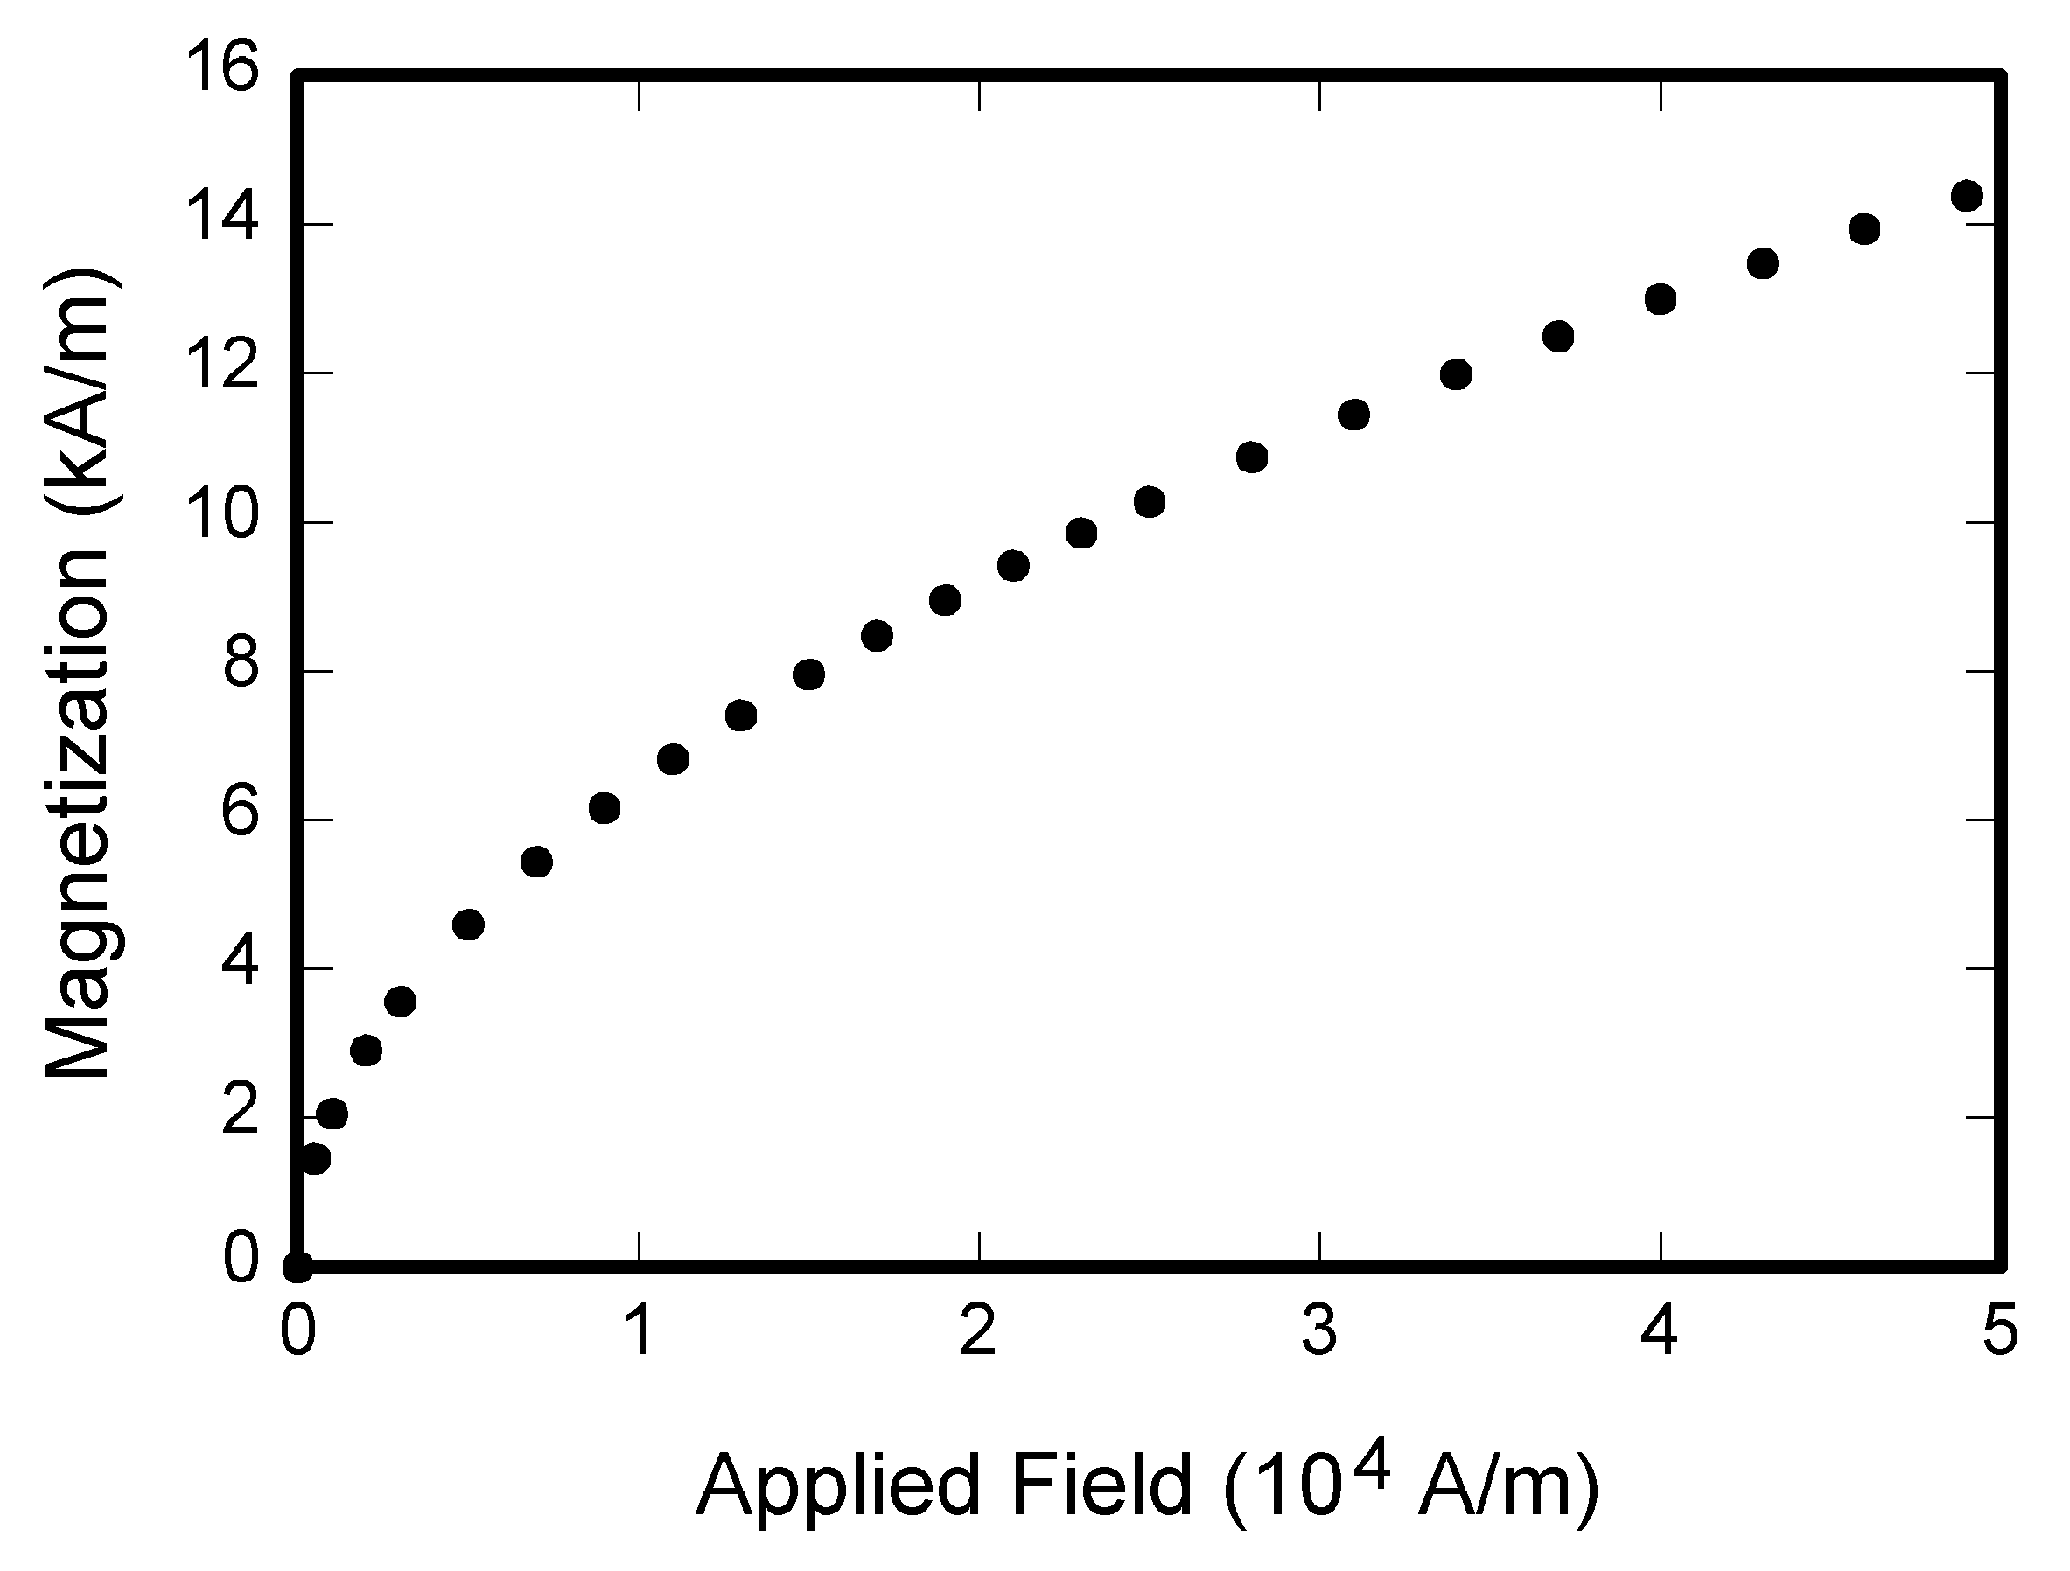
\includegraphics[width=\columnwidth]{fig1.png}}
\caption{Magnetization as a function of applied field.
It is good practice to explain the significance of the figure in the caption.}
\label{fig1}
\end{figure}

Be aware of the different meanings of the homophones ``affect'' (usually a 
verb) and ``effect'' (usually a noun), ``complement'' and ``compliment,'' 
``discreet'' and ``discrete,'' ``principal'' (e.g., ``principal 
investigator'') and ``principle'' (e.g., ``principle of measurement''). Do 
not confuse ``imply'' and ``infer.'' 

Prefixes such as ``non,'' ``sub,'' ``micro,'' ``multi,'' and ``ultra'' are 
not independent words; they should be joined to the words they modify, 
usually without a hyphen. There is no period after the ``et'' in the Latin 
abbreviation ``\emph{et al.}'' (it is also italicized). The abbreviation ``i.e.,'' means 
``that is,'' and the abbreviation ``e.g.,'' means ``for example'' (these 
abbreviations are not italicized).

IEEE styleguides are available at
https://journals.\discretionary{}{}{}ieeeauthorcenter.ieee.org/create-your-ieee-journal-article/\discretionary{}{}{}create-the-text-of-your-article/\discretionary{}{}{}ieee-editorial-style-manual/.

\section{Guidelines for Graphics Preparation and Submission}
\label{sec:guidelines}

\subsection{Types of Graphics}
The following list outlines the different types of graphics published in 
IEEE journals. They are categorized based on their construction, and use of 
color/shades of gray:

\subsubsection{Color/Grayscale figures}
{Figures that are meant to appear in color, or shades of black/gray. Such 
figures may include photographs, illustrations, multicolor graphs, and 
flowcharts.}

\subsubsection{Line Art figures}
{Figures that are composed of only black lines and shapes. These figures 
should have no shades or half-tones of gray, only black and white.}

\subsubsection{Author photos}
{Head and shoulders shots of authors that appear at the end of our papers. }

\subsubsection{Tables}
{Data charts which are typically black and white, but sometimes include 
color.}

\begin{table}
\caption{Units for Magnetic Properties}
\label{table}
\setlength{\tabcolsep}{3pt}
\begin{tabular}{|p{25pt}|p{75pt}|p{115pt}|}
\hline
Symbol& 
Quantity& 
Conversion from Gaussian and \par CGS EMU to SI $^{\mathrm{a}}$ \\
\hline
$\Phi $& 
magnetic flux& 
1 Mx $\to  10^{-8}$ Wb $= 10^{-8}$ V$\cdot $s \\
$B$& 
magnetic flux density, \par magnetic induction& 
1 G $\to  10^{-4}$ T $= 10^{-4}$ Wb/m$^{2}$ \\
$H$& 
magnetic field strength& 
1 Oe $\to  10^{3}/(4\pi )$ A/m \\
$m$& 
magnetic moment& 
1 erg/G $=$ 1 emu \par $\to 10^{-3}$ A$\cdot $m$^{2} = 10^{-3}$ J/T \\
$M$& 
magnetization& 
1 erg/(G$\cdot $cm$^{3}) =$ 1 emu/cm$^{3}$ \par $\to 10^{3}$ A/m \\
4$\pi M$& 
magnetization& 
1 G $\to  10^{3}/(4\pi )$ A/m \\
$\sigma $& 
specific magnetization& 
1 erg/(G$\cdot $g) $=$ 1 emu/g $\to $ 1 A$\cdot $m$^{2}$/kg \\
$j$& 
magnetic dipole \par moment& 
1 erg/G $=$ 1 emu \par $\to 4\pi \times  10^{-10}$ Wb$\cdot $m \\
$J$& 
magnetic polarization& 
1 erg/(G$\cdot $cm$^{3}) =$ 1 emu/cm$^{3}$ \par $\to 4\pi \times  10^{-4}$ T \\
$\chi , \kappa $& 
susceptibility& 
1 $\to  4\pi $ \\
$\chi_{\rho }$& 
mass susceptibility& 
1 cm$^{3}$/g $\to  4\pi \times  10^{-3}$ m$^{3}$/kg \\
$\mu $& 
permeability& 
1 $\to  4\pi \times  10^{-7}$ H/m \par $= 4\pi \times  10^{-7}$ Wb/(A$\cdot $m) \\
$\mu_{r}$& 
relative permeability& 
$\mu \to \mu_{r}$ \\
$w, W$& 
energy density& 
1 erg/cm$^{3} \to  10^{-1}$ J/m$^{3}$ \\
$N, D$& 
demagnetizing factor& 
1 $\to  1/(4\pi )$ \\
\hline
\multicolumn{3}{p{251pt}}{Vertical lines are optional in tables. Statements that serve as captions for 
the entire table do not need footnote letters. }\\
\multicolumn{3}{p{251pt}}{$^{\mathrm{a}}$Gaussian units are the same as cg emu for magnetostatics; Mx 
$=$ maxwell, G $=$ gauss, Oe $=$ oersted; Wb $=$ weber, V $=$ volt, s $=$ 
second, T $=$ tesla, m $=$ meter, A $=$ ampere, J $=$ joule, kg $=$ 
kilogram, H $=$ henry.}
\end{tabular}
\label{tab1}
\end{table}

\subsection{Multipart figures}
Figures compiled of more than one sub-figure presented side-by-side, or 
stacked. If a multipart figure is made up of multiple figure
types (one part is lineart, and another is grayscale or color) the figure 
should meet the stricter guidelines.

\subsection{File Formats For Graphics}\label{formats}
Format and save your graphics using a suitable graphics processing program 
that will allow you to create the images as PostScript (PS), Encapsulated 
PostScript (.EPS), Tagged Image File Format (.TIFF), Portable Document 
Format (.PDF), Portable Network Graphics (.PNG), or Metapost (.MPS), sizes them, and adjusts 
the resolution settings. When 
submitting your final paper, your graphics should all be submitted 
individually in one of these formats along with the manuscript.

\subsection{Sizing of Graphics}
Most charts, graphs, and tables are one column wide (3.5 inches/88 
millimeters/21 picas) or page wide (7.16 inches/181 millimeters/43 
picas). The maximum depth a graphic can be is 8.5 inches (216 millimeters/54
picas). When choosing the depth of a graphic, please allow space for a 
caption. Figures can be sized between column and page widths if the author 
chooses, however it is recommended that figures are not sized less than 
column width unless when necessary. 

There is currently one publication with column measurements that do not 
coincide with those listed above. Proceedings of the IEEE has a column 
measurement of 3.25 inches (82.5 millimeters/19.5 picas). 

The final printed size of author photographs is exactly
1 inch wide by 1.25 inches tall (25.4 millimeters$\,\times\,$31.75 millimeters/6 
picas$\,\times\,$7.5 picas). Author photos printed in editorials measure 1.59 inches 
wide by 2 inches tall (40 millimeters$\,\times\,$50 millimeters/9.5 picas$\,\times\,$12 
picas).

\subsection{Resolution }
The proper resolution of your figures will depend on the type of figure it 
is as defined in the ``Types of Figures'' section. Author photographs, 
color, and grayscale figures should be at least 300dpi. Line art, including 
tables should be a minimum of 600dpi.

\subsection{Vector Art}
In order to preserve the figures' integrity across multiple computer 
platforms, we accept files in the following formats: .EPS/.PDF/.PS. All 
fonts must be embedded or text converted to outlines in order to achieve the 
best-quality results.

\subsection{Color Space}
The term color space refers to the entire sum of colors that can be 
represented within the said medium. For our purposes, the three main color 
spaces are Grayscale, RGB (red/green/blue) and CMYK 
(cyan/magenta/yellow/black). RGB is generally used with on-screen graphics, 
whereas CMYK is used for printing purposes.

All color figures should be generated in RGB or CMYK color space. Grayscale 
images should be submitted in Grayscale color space. Line art may be 
provided in grayscale OR bitmap colorspace. Note that ``bitmap colorspace'' 
and ``bitmap file format'' are not the same thing. When bitmap color space 
is selected, .TIF/.TIFF/.PNG are the recommended file formats.

\subsection{Accepted Fonts Within Figures}
When preparing your graphics IEEE suggests that you use of one of the 
following Open Type fonts: Times New Roman, Helvetica, Arial, Cambria, and 
Symbol. If you are supplying EPS, PS, or PDF files all fonts must be 
embedded. Some fonts may only be native to your operating system; without 
the fonts embedded, parts of the graphic may be distorted or missing.

A safe option when finalizing your figures is to strip out the fonts before 
you save the files, creating ``outline'' type. This converts fonts to 
artwork what will appear uniformly on any screen.

\subsection{Using Labels Within Figures}

\subsubsection{Figure Axis labels }
Figure axis labels are often a source of confusion. Use words rather than 
symbols. As an example, write the quantity ``Magnetization,'' or 
``Magnetization M,'' not just ``M.'' Put units in parentheses. Do not label 
axes only with units. As in Fig. 1, for example, write ``Magnetization 
(A/m)'' or ``Magnetization (A$\cdot$m$^{-1}$),'' not just ``A/m.'' Do not label axes with a ratio of quantities and 
units. For example, write ``Temperature (K),'' not ``Temperature/K.'' 

Multipliers can be especially confusing. Write ``Magnetization (kA/m)'' or 
``Magnetization (10$^{3}$ A/m).'' Do not write ``Magnetization 
(A/m)$\,\times\,$1000'' because the reader would not know whether the top 
axis label in Fig. 1 meant 16000 A/m or 0.016 A/m. Figure labels should be 
legible, approximately 8 to 10 point type.

\subsubsection{Subfigure Labels in Multipart Figures and Tables}
Multipart figures should be combined and labeled before final submission. 
Labels should appear centered below each subfigure in 8 point Times New 
Roman font in the format of (a) (b) (c). 

\subsection{File Naming}
Figures (line artwork or photographs) should be named starting with the 
first 5 letters of the author's last name. The next characters in the 
filename should be the number that represents the sequential 
location of this image in your article. For example, in author 
``Anderson's'' paper, the first three figures would be named ander1.tif, 
ander2.tif, and ander3.ps.

Tables should contain only the body of the table (not the caption) and 
should be named similarly to figures, except that `.t' is inserted 
in-between the author's name and the table number. For example, author 
Anderson's first three tables would be named ander.t1.tif, ander.t2.ps, 
ander.t3.eps.

Author photographs should be named using the first five characters of the 
pictured author's last name. For example, four author photographs for a 
paper may be named: oppen.ps, moshc.tif, chen.eps, and duran.pdf.

If two authors or more have the same last name, their first initial(s) can 
be substituted for the fifth, fourth, third$\ldots$ letters of their surname 
until the degree where there is differentiation. For example, two authors 
Michael and Monica Oppenheimer's photos would be named oppmi.tif, and 
oppmo.eps.

\subsection{Referencing a Figure or Table Within Your Paper}
When referencing your figures and tables within your paper, use the 
abbreviation ``Fig.'' even at the beginning of a sentence. Do not abbreviate 
``Table.'' Tables should be numbered with Roman Numerals.

\subsection{Submitting Your Graphics}
Because IEEE will do the final formatting of your paper,
you do not need to position figures and tables at the top and bottom of each 
column. In fact, all figures, figure captions, and tables can be placed at 
the end of your paper. In addition to, or even in lieu of submitting figures 
within your final manuscript, figures should be submitted individually, 
separate from the manuscript in one of the file formats listed above in 
Section \ref{formats}. Place figure captions below the figures; place table titles 
above the tables. Please do not include captions as part of the figures, or 
put them in ``text boxes'' linked to the figures. Also, do not place borders 
around the outside of your figures.

\subsection{Color Processing/Printing in IEEE Journals}
All IEEE Transactions, Journals, and Letters allow an author to publish color figures on IEEE Xplore at no charge, and automatically convert them to grayscale for print versions. In most journals, figures and tables may alternatively be printed in color if an author chooses to do so. Please note that this service comes at an extra expense to the author. If you intend to have print color graphics, you will have the opportunity to indicate this in the Author Gateway and will be contacted by PubOps to confirm the charges. Online-only journals will have their figures appear in color, free of charge 

\section{Conclusion}
A conclusion section is not required. Although a conclusion may review the 
main points of the paper, do not replicate the abstract as the conclusion. A 
conclusion might elaborate on the importance of the work or suggest 
applications and extensions. 

\appendices

Appendixes, if needed, appear before the acknowledgment.

\section*{References and Footnotes}

\subsection{References}
References need not be cited in text. When they are, they appear on the
line, in square brackets, inside the punctuation. Multiple references are
each numbered with separate brackets. When citing a section in a book,
please give the relevant page numbers. In text, refer simply to the
reference number. Do not use ``Ref.'' or ``reference'' except at the
beginning of a sentence: ``Reference [3] shows \textellipsis .'' Please do not use
automatic endnotes in \textit{Word}, rather, type the reference list at the end of the
paper using the ``References'' style.

Reference numbers are set flush left and form a column of their own, hanging
out beyond the body of the reference. The reference numbers are on the line,
enclosed in square brackets. In all references, the given name of the author
or editor is abbreviated to the initial only and precedes the last name. Use
them all; use \textit{et al}.\ only if names are not given.
Abbreviate conference titles. When citing IEEE Transactions,
provide the issue number, page range, volume number, year, and/or month if
available. When referencing a patent, provide the day and the month of
issue, or application. References may not include all information; please
obtain and include relevant information. Do not combine references. There
must be only one reference with each number. If there is a URL included with
the print reference, it can be included at the end of the reference.

Other than books, capitalize only the first word in a paper title, except
for proper nouns and element symbols. For papers published in translation
journals, please give the English citation first, followed by the original
foreign-language citation. See the end of this document for formats and
examples of common references. For a complete discussion of references and
their formats, see the IEEE style manual at 
https://\discretionary{}{}{}journals.ieeeauthorcenter.ieee.org/\discretionary{}{}{}create-your-ieee-journal-article/\discretionary{}{}{}create-the-text-of-your-article/\discretionary{}{}{}ieee-editorial-style-manual/.


\subsection{Footnotes}
Number footnotes separately in superscript numbers.\footnote{It is recommended that footnotes be avoided (except for 
the unnumbered footnote with the receipt date on the first page). Instead, 
try to integrate the footnote information into the text.} Place the actual 
footnote at the bottom of the column in which it is cited; do not put 
footnotes in the reference list (endnotes). Use letters for table footnotes 
(see Table \ref{table}).

\section*{Submitting Your Paper for Review}           

\subsection{Review Stage Using IEEE ScholarOne Manuscripts}

Contributions to the Transactions, Journals, and Letters may be submitted electronically on IEEE ScholarOne Manuscripts. You can get help choosing the correct publication for your manuscript as well as find their corresponding peer review site using the tools listed at http://\discretionary{}{}{}www.ieee.org/\discretionary{}{}{}publications\_standards/\discretionary{}{}{}publications/\discretionary{}{}{}authors/\discretionary{}{}{}authors\_submission.html. Once you have chosen your publication and navigated to the IEEE ScholarOne Manuscripts site, you may log in with your IEEE web account. If there is none, please create a new account. After logging in, go to your Author Center and click ``Start New Submission.''

Along with other information, you will be asked to select the manuscript type from the journal's pre-determined list of options. Depending on the journal, there are various steps to the submission process; please make sure to carefully answer all of the submission questions presented to you. At the end of each step you must click ``Save and Continue''; just uploading the paper is not sufficient. After the last step, you should see a confirmation that the submission is complete. You should also receive an e-mail confirmation. For inquiries regarding the submission of your paper on IEEE ScholarOne Manuscripts, please contact oprs-support@ieee.org or call +1 732 465 5861.

IEEE ScholarOne Manuscripts will accept files for review in various formats. There is a ``Journal Home'' link on the log-in page of each IEEE ScholarOne Manuscripts site that will bring you to the journal's homepage with their detailed requirements; please check these guidelines for your particular journal before you submit.

\subsection{Final Stage Using IEEE ScholarOne Manuscripts}
Upon acceptance, you will receive an email with specific instructions
regarding the submission of your final files. To avoid any delays in
publication, please be sure to follow these instructions. Most journals
require that final submissions be uploaded through IEEE ScholarOne Manuscripts,
although some may still accept final submissions via email. Final
submissions should include source files of your accepted manuscript, high
quality graphic files, and a formatted pdf file. If you have any questions
regarding the final submission process, please contact the administrative
contact for the journal.

In addition to this, upload a file with complete contact information for all
authors. Include full mailing addresses, telephone numbers, fax numbers, and
e-mail addresses. Designate the author who submitted the manuscript on
IEEE ScholarOne Manuscripts as the ``corresponding author.'' This is the only
author to whom proofs of the paper will be sent.

\subsection{Copyright Form}
Authors must submit an electronic IEEE Copyright Form (eCF) upon submitting 
their final manuscript files. You can access the eCF system through your 
manuscript submission system or through the Author Gateway. You are 
responsible for obtaining any necessary approvals and/or security 
clearances. For additional information on intellectual property rights, 
visit the IEEE Intellectual Property Rights department web page at 
\underline{http://www.ieee.org/publications\_standards/publications/rights/}\discretionary{}{}{}\underline{index.html}.

\section*{IEEE Publishing Policy}
The general IEEE policy requires that authors should only submit original 
work that has neither appeared elsewhere for publication, nor is under 
review for another refereed publication. The submitting author must disclose 
all prior publication(s) and current submissions when submitting a 
manuscript. Do not publish ``preliminary'' data or results. The submitting 
author is responsible for obtaining agreement of all coauthors and any 
consent required from employers or sponsors before submitting an article. 
The IEEE Transactions and Journals Department strongly discourages courtesy 
authorship; it is the obligation of the authors to cite only relevant prior 
work.

The IEEE Transactions and Journals Department does not publish conference 
records or proceedings, but can publish articles related to conferences that 
have undergone rigorous peer review. Minimally, two reviews are required for 
every article submitted for peer review.

\section*{Acknowledgment}

The preferred spelling of the word ``acknowledgment'' in American English is 
without an ``e'' after the ``g.'' Use the singular heading even if you have 
many acknowledgments. Avoid expressions such as ``One of us (S.B.A.) would 
like to thank $\ldots$ .'' Instead, write ``F. A. Author thanks $\ldots$ .'' In most 
cases, sponsor and financial support acknowledgments are placed in the 
unnumbered footnote on the first page, not here.

\section*{References}

\def\refname{\vadjust{\vspace*{-2.5em}}} %Please don't do this in a real paper.

\noindent\textit{Basic format for books:}

\noindent J. K. Author, ``Title of chapter in the book,'' in {\it Title of His Published Book, x}th ed. City of Publisher,
(only U.S. State), Country: Abbrev. of Publisher, year, ch. $x$, sec. $x$,\break pp.~{\it xxx--xxx.}

{\it Examples:}{\vadjust{\vspace*{-2.5em}}}
\begin{thebibliography}{00}
\bibitem{bib1} G. O. Young, ``Synthetic structure of industrial plastics,'' in {\it Plastics,}2$^{\mathrm{nd}}$ ed., vol. 3, J. Peters, Ed. New York, NY, USA: McGraw-Hill, 1964, pp. 15--64.
\bibitem{bib2} W.-K. Chen, {\it Linear Networks and Systems.}Belmont, CA, USA: Wadsworth, 1993, pp. 123--135.
\end{thebibliography}

\noindent {\it Basic format for periodicals:}

\noindent J. K. Author, ``Name of paper,'' {\it Abbrev. Title of Periodical}, vol. {\it x, no}. $x, $pp{\it . xxx-xxx,}Abbrev. Month, year, DOI.
 {10.1109.} {{\it XXX}} {.123456}.

{\it Examples:}{\vadjust{\vspace*{-2.5em}}}

\begin{thebibliography}{00}\leftskip1pc
\bibitem{bib3} J. U. Duncombe, ``Infrared navigation---Part I: An assessment of feasibility,'' {\it IEEE Trans. Electron Devices}, vol. ED-11, no. 1, pp. 34--39, Jan. 1959, doi:.  {10.1109/TED.2016.2628402}.
\bibitem{bib4} E. P. Wigner, ``Theory of traveling-wave optical laser,''
{\it Phys. Rev}., vol. 134, pp. A635--A646, Dec. 1965, doi:  {10.1109.} {{\it XXX}} {.123456}.
\bibitem{bib5} E. H. Miller, ``A note on reflector arrays,'' {\it IEEE Trans. Antennas Propagat}., to be published.
\end{thebibliography}

\noindent {\it Basic format for reports:}

\noindent J. K. Author, ``Title of report,'' Abbrev. Name of Co., City of Co., Abbrev.
State, Country, Rep. {\it xxx}, year.

{\it Examples:}
\begin{thebibliography}{00}\leftskip1pc
\bibitem{bib6} E. E. Reber, R. L. Michell, and C. J. Carter, ``Oxygen absorption in the earth's atmosphere,'' Aerospace Corp., Los Angeles, CA, USA, Tech. Rep. TR-0200 (4230-46)-3, Nov. 1988.
\bibitem{bib7} J. H. Davis and J. R. Cogdell, ``Calibration program for the 16-foot antenna,'' Elect. Eng. Res. Lab., Univ. Texas, Austin, TX, USA, Tech. Memo. NGL-006-69-3, Nov. 15, 1987.
\end{thebibliography}

\noindent {\it Basic format for handbooks:}

\noindent {\it Name of Manual/Handbook, x} ed., Abbrev. Name of Co., City of Co., Abbrev. State, Country, year, pp.
{\it xxx-xxx.}

{\it Examples:}{\vadjust{\vspace*{-2.5em}}}

\begin{thebibliography}{00}\leftskip1pc
\bibitem{bib8} {\it Transmission Systems for Communications}, 3rd ed., Western Electric Co., Winston-Salem, NC, USA, 1985, pp. 44--60.
\bibitem{bib9} {\it Motorola Semiconductor Data Manual}, Motorola Semiconductor Products Inc., Phoenix, AZ, USA, 1989.
\end{thebibliography}

\noindent {\it Basic format for books (when available online):}

\noindent J. K. Author, ``Title of chapter in the book,'' in {\it Title of Published Book}, $x$th ed. City of
Publisher, State, Country: Abbrev. of Publisher, year, ch.$x$, sec. $x$, pp.
{\it xxx--xxx}. [Online]. Available:  {http://www.web.com}




{\it Examples:}{\vadjust{\vspace*{-2.5em}}}

\begin{thebibliography}{00}\leftskip1pc
\bibitem{bib10} G. O. Young, ``Synthetic structure of industrial plastics,'' in Plastics, vol. 3, Polymers of Hexadromicon, J. Peters, Ed., 2nd ed. New York, NY, USA: McGraw-Hill, 1964, pp. 15-64. [Online]. Available:  {http://www.bookref.com}.
\bibitem{bib11} {\it The Founders' Constitution}, Philip B. Kurland and Ralph Lerner, eds., Chicago, IL, USA: Univ. Chicago Press, 1987. [Online]. Available:  {http://press-pubs.uchicago.edu/founders/}
\bibitem{bib12} The Terahertz Wave eBook. ZOmega Terahertz Corp., 2014. [Online]. Available:  {http://dl.z-thz.com/eBook/zomega\_ebook\_pdf\_1206\_sr.pdf}. Accessed on: May 19, 2014.
\bibitem{bib13} Philip B. Kurland and Ralph Lerner, eds., {\it The Founders' Constitution.}Chicago, IL, USA: Univ. of Chicago Press, 1987, Accessed on: Feb. 28, 2010, [Online] Available:  {http://press-pubs.uchicago.edu/founders/}
\end{thebibliography}

\noindent {\it Basic format for journals (when available online):}

\noindent J. K. Author, ``Name of paper,'' {\it Abbrev. Title of Periodical}, vol. $x$, no. $x$, pp. {\it xxx-xxx}, Abbrev. Month, year.
Accessed on: Month, Day, year, doi:  {10.1109.} {{\it
XXX}} {.123456}, [Online].

{\it Examples:}{\vadjust{\vspace*{-2.5em}}}

\begin{thebibliography}{00}\leftskip1pc
\bibitem{bib14} J. S. Turner, ``New directions in communications,'' {\it IEEE J. Sel. Areas Commun}., vol. 13, no. 1, pp. 11-23, Jan. 1995. DOI.  {10.1109.} {{\it XXX}} {.123456}.
\bibitem{bib15} W. P. Risk, G. S. Kino, and H. J. Shaw, ``Fiber-optic frequency shifter using a surface acoustic wave incident at an oblique angle,'' {\it Opt. Lett.}, vol. 11, no. 2, pp. 115--117, Feb. 1986, doi: {10.1109.} {{\it XXX}} {.123456}.
\bibitem{bib16} P. Kopyt {\it \textit{et al.}, ``}Electric properties of graphene-based conductive layers from DC up to terahertz range,'' {\it IEEE THz Sci. Technol.,}to be published, doi:  {10.1109/TTHZ.2016.2544142}.
\end{thebibliography}

\noindent {\it Basic format for papers presented at conferences (when available online):}

\noindent J.K. Author. (year, month). Title. presented at abbrev. conference title.
[Type of Medium]. Available: site/path/file
\\
\\
\\
{\it Example:}{\vadjust{\vspace*{-2.5em}}}

\begin{thebibliography}{00}\leftskip1pc
\bibitem{bib17} PROCESS Corporation, Boston, MA, USA. Intranets: Internet technologies deployed behind the firewall for corporate productivity. Presented at INET96 Annual Meeting. [Online]. Available:  {http://home.process.com/Intranets/wp2.htp}
\end{thebibliography}

\noindent {\it Basic format for reports and handbooks (when available online):}

\noindent J. K. Author. ``Title of report,'' Company. City, State, Country. Rep. no.,
(optional: vol./issue), Date. [Online] Available:\\
{site/path/file}\\

{\it Examples:}{\vadjust{\vspace*{-2.5em}}}

\begin{thebibliography}{00}\leftskip1pc
\bibitem{bib18} R. J. Hijmans and J. van Etten, ``Raster: Geographic analysis and modeling with raster data,'' R Package Version 2.0-12, Jan. 12, 2012. [Online]. Available:  {http://CRAN.R-project.org/package$=$raster} {}
\bibitem{bib19} Teralyzer. Lytera UG, Kirchhain, Germany [Online]. Available: http://www.lytera.de/Terahertz\_THz\_Spectroscopy.php?id$=$home, Accessed on: Jun. 5, 2014
\end{thebibliography}

\noindent {\it Basic format for computer programs and electronic documents (when available online):}

\noindent Legislative body. Number of Congress, Session. (year, month day). {\it Number of bill or resolution}, {\it Title}. [Type
of medium]. Available: site/path/file

\noindent {\bf {\it NOTE:}} ISO recommends that capitalization follow the accepted
practice for the language or script in which the information is given.



{\it Example:}{\vadjust{\vspace*{-2.5em}}}

\begin{thebibliography}{00}\leftskip1pc
\bibitem{bib20} U.S. House. 102nd Congress, 1st Session. (1991, Jan. 11). {\it H. Con. Res. 1, Sense of the Congress on Approval of Military Action}. [Online]. Available: LEXIS Library: GENFED File: BILLS
\end{thebibliography}

\noindent {\it Basic format for patents (when available online):}

\noindent Name of the invention, by inventor's name. (year, month day). Patent Number  [Type
of medium]. Available:  {site/path/file}

{\it Example:}{\vadjust{\vspace*{-2.5em}}}

\begin{thebibliography}{00}\leftskip1pc
\bibitem{bib21} Musical toothbrush with mirror, by L.M.R. Brooks. (1992, May 19). Patent D 326 189 [Online]. Available: NEXIS Library: LEXPAT File: DES
\end{thebibliography}


\noindent {\it Basic format for conference proceedings (published):}

\noindent J. K. Author, ``Title of paper,'' in {\it Abbreviated Name of Conf.}, City of Conf., Abbrev. State (if
given), Country, year, pp. {\it xxxxxx.}

{\it Example:}{\vadjust{\vspace*{-2.5em}}}

\begin{thebibliography}{00}\leftskip1pc
\bibitem{bib22} D. B. Payne and J. R. Stern, ``Wavelength-switched passively coupled single-mode optical network,'' in {\it Proc. IOOC-ECOC,}Boston, MA, USA,  1985,
pp. 585--590, doi:  {10.1109.} {{\it XXX}} {.123456}.
\end{thebibliography}

{\it Example for papers presented at conferences (unpublished):}{\vadjust{\vspace*{-2.5em}}}

\begin{thebibliography}{00}\leftskip1pc
\bibitem{bib23} D. Ebehard and E. Voges, ``Digital single sideband detection for interferometric sensors,'' presented at the {\it 2nd Int. Conf. Optical Fiber Sensors,} Stuttgart, Germany, Jan. 2-5, 1984.
\end{thebibliography}

\noindent {\it Basic format for patents:}

\noindent J. K. Author, ``Title of patent,'' U.S. Patent {\it x xxx xxx}, Abbrev. Month, day, year.

{\it Example:}{\vadjust{\vspace*{-2.5em}}}

\begin{thebibliography}{00}\leftskip1pc
\bibitem{bib24} G. Brandli and M. Dick, ``Alternating current fed power supply,'' U.S. Patent 4 084 217, Nov. 4, 1978.
\end{thebibliography}

\noindent {\it Basic format} {\it for theses (M.S.) and dissertations (Ph.D.):}

\noindent a) J. K. Author, ``Title of thesis,'' M.S. thesis, Abbrev. Dept., Abbrev.
Univ., City of Univ., Abbrev. State, year.

\noindent b) J. K. Author, ``Title of dissertation,'' Ph.D. dissertation, Abbrev.
Dept., Abbrev. Univ., City of Univ., Abbrev. State, year.

{\it Examples:}{\vadjust{\vspace*{-2.5em}}}

\begin{thebibliography}{00}\leftskip1pc
\bibitem{bib25} J. O. Williams, ``Narrow-band analyzer,'' Ph.D. dissertation, Dept. Elect. Eng., Harvard Univ., Cambridge, MA, USA, 1993.
\bibitem{bib26} N. Kawasaki, ``Parametric study of thermal and chemical nonequilibrium nozzle flow,'' M.S. thesis, Dept. Electron. Eng., Osaka Univ., Osaka, Japan, 1993.
\end{thebibliography}

\noindent {\it Basic format for the most common types of unpublished references:}

\noindent a) J. K. Author, private communication, Abbrev. Month, year.

\noindent b) J. K. Author, ``Title of paper,'' unpublished.

\noindent c) J. K. Author, ``Title of paper,'' to be published.

{\it Examples:}{\vadjust{\vspace*{-2.5em}}}

\begin{thebibliography}{00}\leftskip1pc
\bibitem{bib27} A. Harrison, private communication, May 1995.
\bibitem{bib28} B. Smith, ``An approach to graphs of linear forms,'' unpublished.
\bibitem{bib29} A. Brahms, ``Representation error for real numbers in binary computer arithmetic,'' IEEE Computer Group Repository, Paper R-67-85.
\end{thebibliography}

\noindent {\it Basic formats for standards:}

\noindent a) {\it Title of Standard}, Standard number, date.

\noindent b) {\it Title of Standard}, Standard number, Corporate author, location, date.

{\it Examples:}{\vadjust{\vspace*{-2.5em}}}

\begin{thebibliography}{00}\leftskip1pc
\bibitem{bib30} IEEE Criteria for Class IE Electric Systems, IEEE Standard 308, 1969.
\bibitem{bib31} Letter Symbols for Quantities, ANSI Standard Y10.5-1968.
\end{thebibliography}

{\it Article number in~reference examples:}{\vadjust{\vspace*{-2.5em}}}

\begin{thebibliography}{00}\leftskip1pc
\bibitem{bib32} R. Fardel, M. Nagel, F. Nuesch, T. Lippert, and A. Wokaun, ``Fabrication of organic light emitting diode pixels by laser-assisted forward transfer,'' {\it Appl. Phys. Lett.}, vol. 91, no. 6, Aug. 2007, Art. no. 061103, doi:  {10.1109.} {{\it XXX}} {.123456}.
\bibitem{bib33} J. Zhang and N. Tansu, ``Optical gain and laser characteristics of InGaN quantum wells on ternary InGaN substrates,'' {\it IEEE Photon. J.}, vol. 5, no. 2, Apr. 2013, Art. no. 2600111, doi:  {10.1109.} {{\it XXX}} {.123456}.
\end{thebibliography}

{\it Example when using \textit{et al.}:}{\vadjust{\vspace*{-2.5em}}}

\begin{thebibliography}{00}\leftskip1pc
\bibitem{bib34} S. Azodolmolky~{{et al.}}, Experimental demonstration of an impairment aware network planning and operation tool for transparent/translucent optical networks,''~{\it J. Lightw. Technol.}, vol. 29, no. 4, pp. 439--448, Sep. 2011,doi:  {10.1109.} {{\it XXX}} {.123456}.
\end{thebibliography}

\noindent {\it Basic format for datasets:}

\noindent Author,  Date, Year. ``Title of Dataset,'' distributed by Publisher/Distributor, http://url.com (or if DOI is used, end with a period)

{\it Example:}{\vadjust{\vspace*{-2.5em}}}

\begin{thebibliography}{00}\leftskip1pc
\bibitem{bib35} U.S. Department of Health and Human Services, Aug. 2013, ``Treatment Episode Dataset: Discharges (TEDS-D): Concatenated, 2006 to 2009,'' U.S. Department of Health and Human Services, Substance Abuse and Mental Health Services Administration, Office of Applied Studies, doi: 10.3886/ICPSR30122.v2.
\end{thebibliography}

\noindent {\it Basic format for code:}

\noindent Author,  Date published or disseminated, Year. ``Complete title, including ed./vers.\#,'' distributed by Publisher/Distributor, http://url.com (or if DOI is used, end with a period)

{\it Example:}{\vadjust{\vspace*{-2.5em}}}

\begin{thebibliography}{00}\leftskip1pc
\bibitem{bib36} T. D'Martin and S. Soares, 2019, ``Code for Assessment of Markov Decision Processes in Long-Term Hydrothermal Scheduling of Single-Reservoir Systems (Version 1.0),'' Code Ocean, doi: \_1.24433/CO.7212286.v1
\end{thebibliography}

\begin{IEEEbiography}[{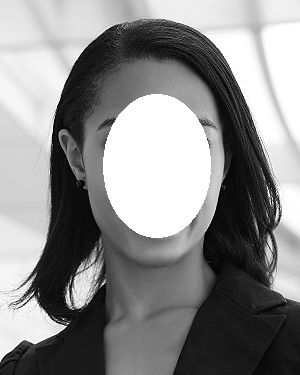
\includegraphics[width=1in,height=1.25in,clip,keepaspectratio]{a1.png}}]{First A. Author} (Fellow, IEEE) and all authors may include 
biographies. Biographies are
often not included in conference-related papers.
This author is an IEEE Fellow. The first paragraph
may contain a place and/or date of birth (list
place, then date). Next, the author’s educational
background is listed. The degrees should be listed
with type of degree in what field, which institution,
city, state, and country, and year the degree was
earned. The author’s major field of study should
be lower-cased.

The second paragraph uses the pronoun of the person (he or she) and
not the author’s last name. It lists military and work experience, including
summer and fellowship jobs. Job titles are capitalized. The current job must
have a location; previous positions may be listed without one. Information
concerning previous publications may be included. Try not to list more than
three books or published articles. The format for listing publishers of a book
within the biography is: title of book (publisher name, year) similar to a
reference. Current and previous research interests end the paragraph.

The third paragraph begins with the author’s title and last name (e.g.,
Dr. Smith, Prof. Jones, Mr. Kajor, Ms. Hunter). List any memberships in
professional societies other than the IEEE. Finally, list any awards and work
for IEEE committees and publications. If a photograph is provided, it should
be of good quality, and professional-looking.
\end{IEEEbiography}

\begin{IEEEbiographynophoto}{Second B. Author,} photograph and biography not available at the
time of publication.
\end{IEEEbiographynophoto}

\begin{IEEEbiographynophoto}{Third C. Author Jr.} (Member, IEEE), photograph and biography not available at the
time of publication.
\end{IEEEbiographynophoto}

\end{document}
